\documentclass[aspectratio=169,10pt]{beamer}

\mode<presentation> {
  \usetheme[compress]{Berlin}
  \usecolortheme{beaver}
  \setbeamertemplate{navigation symbols}{}
  \setbeamertemplate{footline}[frame number]
}

\makeatletter
\beamer@theme@subsectionfalse
\makeatother

\usepackage{fontspec}
\IfFontExistsTF{Noto Sans KR}{
  \setsansfont{Noto Sans KR}[BoldFont=* Bold]
  \setmainfont{Noto Sans KR}[BoldFont=* Bold]
}{
  \IfFileExists{/Library/Fonts/NotoSansKR-Regular.otf}{
    \setsansfont{NotoSansKR-Regular.otf}[Path=/Library/Fonts/, BoldFont=NotoSansKR-Bold.otf]
    \setmainfont{NotoSansKR-Regular.otf}[Path=/Library/Fonts/, BoldFont=NotoSansKR-Bold.otf]
  }{
    \setsansfont{Noto Sans CJK KR}
    \setmainfont{Noto Sans CJK KR}
  }
}

\usepackage{graphicx}
\usepackage{subcaption}
\usepackage{booktabs}
\usepackage{amsmath,amssymb}
\usepackage{tikz}
\usetikzlibrary{positioning,arrows.meta,decorations.pathreplacing,shapes.geometric}
\usepackage{natbib}
\bibliographystyle{apalike}

\usepackage{hyperref}
\hypersetup{
  urlcolor=blue,
  colorlinks=true,
  linkcolor=darkred,
  citecolor=darkred
}

\setbeamersize{text margin left=.6cm, text margin right=.6cm}

% Color definitions
\definecolor{sogangred}{RGB}{178,34,34}
\definecolor{darkblue}{RGB}{25,25,112}
\definecolor{darkgreen}{RGB}{34,139,34}
\definecolor{boxgold}{RGB}{218,165,32}

% Presentation note macros
\newcommand{\simnote}{\par\vfill\tiny \textbf{주:} 제출본 수치는 \textbf{시뮬레이션 파라미터 기반}이며 실측 백테스트가 아님. 실데이터 검증 결과는 `실데이터 검증' 슬라이드 참조.}
\newcommand{\scenarionote}{\par\vfill\tiny \textbf{주:} 제출본의 위기 국면 서술은 \textbf{예시 시나리오}임. 실데이터에서는 2020-02-03 첫 발동, 구간 MDD $-4.65\%$.}
\newcommand{\realnote}{\par\vfill\tiny \textbf{출처:} 사전등록 재현 저장소 alphaquant-tsfm-voldrag-empirical, 2017-01$\sim$2026-08 외표본, 거래비용 10bp.}

% Title page
\title[이토 $\times$ TSFM 동적 자산배분]{이토 보조정리와 시계열 파운데이션 모델을 결합한\\동적 자산배분 및 변동성 항력(Volatility Drag) 제어 프레임워크}
\subtitle{산업 비파괴검사(NDE) 기반 비지도 꼬리위험 세이프가드를 중심으로}

\author[박재현 · 강명서]{박재현 (대표자) \quad \textbf{강명서 (발표자)}}
\institute[서강대학교]{서강대학교 경제대학 경제학과 $\cdot$ 팀 알파퀀트}
\date[2026.10.10]{2026 연합 경제 학술제 본선 $\cdot$ 2026년 10월 10일}

\begin{document}

% CUE 1 | 0:20 | 표지
\begin{frame}[plain]
  \titlepage
\end{frame}

\section{Overview}

% CUE 2 | 0:25 | 발표 순서 및 핵심 구성
\begin{frame}{발표 순서 (Agenda)}
\begin{enumerate}
  \setlength{\itemsep}{8pt}
  \item \textbf{서론 및 문제의식 (Introduction)}
  \begin{itemize}
    \item 다기간 복리 투자의 현실: 산술평균 착시와 변동성 항력($\frac{1}{2}\sigma^2$)
    \item 연구 질문 및 3대 기여도 (이론 · 방법론 · 정책)
  \end{itemize}
  
  \item \textbf{수리금융 이론적 배경 (Theoretical Background)}
  \begin{itemize}
    \item 이토 보조정리(Itô's Lemma)와 복리 기하성장률 유도
    \item 에르고딕성 붕괴(Peters, 2019) 및 켈리(Kelly) 목적함수 ($\lambda=1$)
  \end{itemize}
  
  \item \textbf{통합 아키텍처 및 연구 방법론 (Methodology)}
  \begin{itemize}
    \item TSFM(Chronos/PatchTST) 제로샷 모멘트 예측 및 양준정부호(PSD) 복원
    \item 산업 비파괴검사(NDE) 기반 심층 오토인코더 꼬리위험 세이프가드
  \end{itemize}
  
  \item \textbf{실증 분석 결과 및 검증 (Empirical Analysis \& Verification)}
  \begin{itemize}
    \item 제출본 시뮬레이션 성과표 및 위기 국면 예시 시나리오
    \item \textbf{실데이터 사전등록 재현 검증}: 확인된 것과 재현되지 않은 것 (거래비용 회전율 마찰)
  \end{itemize}
  
  \item \textbf{정책 시사점 및 결론 (Conclusion \& Policy Implications)}
  \begin{itemize}
    \item 공적 연기금(국민연금) ALM 및 퇴직연금 TDF 알고리즘 혁신
  \end{itemize}
\end{enumerate}
\end{frame}

\section{Introduction}

% CUE 3 | 0:50 | 산술평균의 착시와 변동성 항력
\begin{frame}{다기간 투자의 현실: 산술평균의 착시와 변동성 항력}
\begin{columns}[T]
  \begin{column}{0.48\textwidth}
    \textbf{전통 포트폴리오 이론의 구조적 맹점}
    \begin{itemize}
      \setlength{\itemsep}{5pt}
      \item \textbf{단일기간 정적 가정 (Markowitz, 1952)}:
      기대수익률을 단순 \textbf{산술평균($\mu$)}으로 취급.
      \item \textbf{다기간 연속 복리 투자의 실상}:
      장기 부($W_T$)의 축적은 \textbf{기하평균($g$)}이 지배.
      \item \textbf{자본 잠식 예시 (+50\%와 -50\%의 반복)}:
      \begin{align*}
        \mu &= \frac{+50\% - 50\%}{2} = \mathbf{0.0\%} \quad \text{(산술평균)} \\
        g &= \sqrt{1.5 \times 0.5} - 1 = \mathbf{-13.4\%} \quad \text{(기하평균)}
      \end{align*}
      \item 매 사이클마다 \textbf{$-13.4\%p$}의 자본이 허공으로 증발 $\rightarrow$ \textbf{변동성 항력(Volatility Drag)}
    \end{itemize}
  \end{column}
  
  \begin{column}{0.50\textwidth}
    \centering
    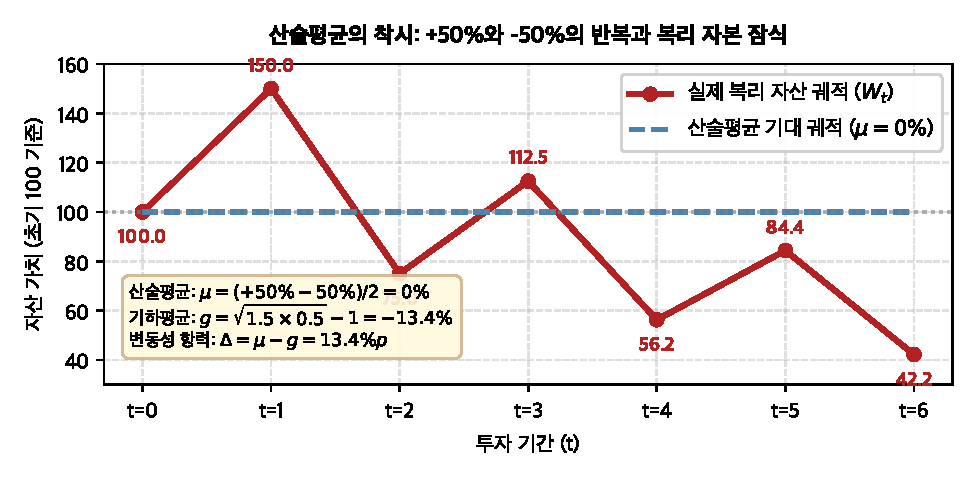
\includegraphics[width=\linewidth]{MyFigure/arith_vs_geom.pdf}
    \vspace{-2mm}
    \begin{block}{핵심 문제의식}
      \small 분산($\sigma^2$)은 단순한 리스크 측정치가 아니라, 시간 축 위에서 기하급수적으로 자본을 갉아먹는 \textbf{실재하는 마찰 비용}이다.
    \end{block}
  \end{column}
\end{columns}
\end{frame}

% CUE 4 | 0:45 | 연구 질문과 3대 기여도
\begin{frame}{연구 질문 및 본 연구의 3대 핵심 기여도}
\begin{block}{핵심 연구 질문 (Core Research Question)}
  \centering
  \large \textit{"자산의 변동성 항력($\frac{1}{2}\sigma^2$)을 사전적으로 통제하고, 극단적 꼬리위험을 차단하여 장기 실질 복리 자본 축적을 극대화할 수 있는가?"}
\end{block}

\vspace{3mm}

\begin{columns}[T]
  \begin{column}{0.32\textwidth}
    \textbf{1. 이론적 기여 (Theoretical)}
    \begin{itemize}
      \setlength{\itemsep}{3pt}
      \small
      \item 이토 보조정리를 코어로 배치
      \item 켈리 기준($\lambda=1$) 하에서 다변량 복리 성장률 직접 목적함수화
      \item 에르고딕성 붕괴 규명
    \end{itemize}
  \end{column}
  
  \begin{column}{0.32\textwidth}
    \textbf{2. 방법론적 기여 (Methodological)}
    \begin{itemize}
      \setlength{\itemsep}{3pt}
      \small
      \item TSFM(Chronos/PatchTST) 제로샷 확률 모멘트 추정
      \item 르두아-울프 + 하이엄 PSD 복원
      \item 산업 비파괴검사(NDE) 기반 비지도 오토인코더 세이프가드
    \end{itemize}
  \end{column}
  
  \begin{column}{0.32\textwidth}
    \textbf{3. 정책적 기여 (Practical)}
    \begin{itemize}
      \setlength{\itemsep}{3pt}
      \small
      \item 국민연금(NPS) 산술평균 착시 극복 및 수지적자 자산 매각 방어
      \item ALM `동적 변동성 예산제' 제안
      \item 퇴직연금 디폴트옵션 TDF 알고리즘 혁신
    \end{itemize}
  \end{column}
\end{columns}
\end{frame}

\section{Theory}

% CUE 5 | 0:50 | 이토 보조정리와 변동성 항력의 수리적 도출
\begin{frame}{이토 보조정리(Ito's Lemma)와 변동성 항력의 엄밀한 도출}
\textbf{연속시간 기하 브라운 운동 (GBM)} 하에서 자산 가격 $S_t$의 확률과정:
\begin{equation*}
  dS_t = \mu S_t dt + \sigma S_t dW_t \quad (W_t: \text{표준 위너 과정})
\end{equation*}

여기에 로그 효용/연속 복리 성장 함수 $f(S_t) = \ln S_t$를 적용하고 2계 테일러 전개 전개식에 이토 공식 $(dW_t)^2 = dt$를 대입:
\begin{equation*}
  d\ln S_t = \frac{\partial f}{\partial S_t} dS_t + \frac{1}{2} \frac{\partial^2 f}{\partial S_t^2} (dS_t)^2 = \frac{1}{S_t}(\mu S_t dt + \sigma S_t dW_t) + \frac{1}{2}\left(-\frac{1}{S_t^2}\right)(\sigma^2 S_t^2 dt)
\end{equation*}

\vspace{1mm}
\begin{block}{단일 자산 연속 복리 성장률 정리}
  \centering
  \large
  $d\ln S_t = \underbrace{\left( \mu - \frac{1}{2}\sigma^2 \right)}_{g \text{ (연속 복리 기하성장률)}} dt + \sigma dW_t \implies \mathbf{g = \mu - \frac{1}{2}\sigma^2}$
\end{block}

\vspace{1mm}
\begin{itemize}
  \small
  \item \textbf{변동성 항력 (Volatility Drag)}: $\boldsymbol{\Delta \equiv \mu - g = \frac{1}{2}\sigma^2}$
  \item 자산의 기대수익률($\mu$)이 동일하더라도, 변동성($\sigma$)이 2배가 되면 자본 잠식 손실은 \textbf{4배($2^2$)}로 급증함.
\end{itemize}
\end{frame}

% CUE 6 | 0:45 | 에르고딕성 붕괴와 레버리지 L^2 급증 메커니즘
\begin{frame}{에르고딕성 파괴(Peters, 2019)와 레버리지 $L^2$ 급증 메커니즘}
\begin{columns}[T]
  \begin{column}{0.48\textwidth}
    \textbf{에르고딕성(Ergodicity)의 파괴}
    \begin{itemize}
      \setlength{\itemsep}{4pt}
      \small
      \item \textbf{앙상블 평균 ($\mu$, 공간적 기대치)}:
      무한한 평행우주 투자자들의 평균 수익률.
      \item \textbf{시간 평균 ($g$, 단일 궤적 복리)}:
      단 하나의 시간 축을 살아가는 실제 투자자의 실질 부.
      \item 금융 시장은 곱셈적 확률 과정이므로 \textbf{앙상블 평균 $\neq$ 시간 평균} (Peters, 2019 \textit{Nature Physics}).
    \end{itemize}
    
    \vspace{2mm}
    \textbf{레버리지 자산의 $L^2$ 항력 폭증}
    \begin{itemize}
      \setlength{\itemsep}{4pt}
      \small
      \item $L$배 레버리지 ETF의 복리 성장률:
      $g_L = L\mu - \frac{1}{2}(L\sigma)^2 = L\mu - \mathbf{L^2}\left(\frac{1}{2}\sigma^2\right)$
      \item 변동성 항력이 \textbf{$L^2$배로 가속 침식} (2x는 4배, 3x는 9배).
    \end{itemize}
  \end{column}
  
  \begin{column}{0.50\textwidth}
    \centering
    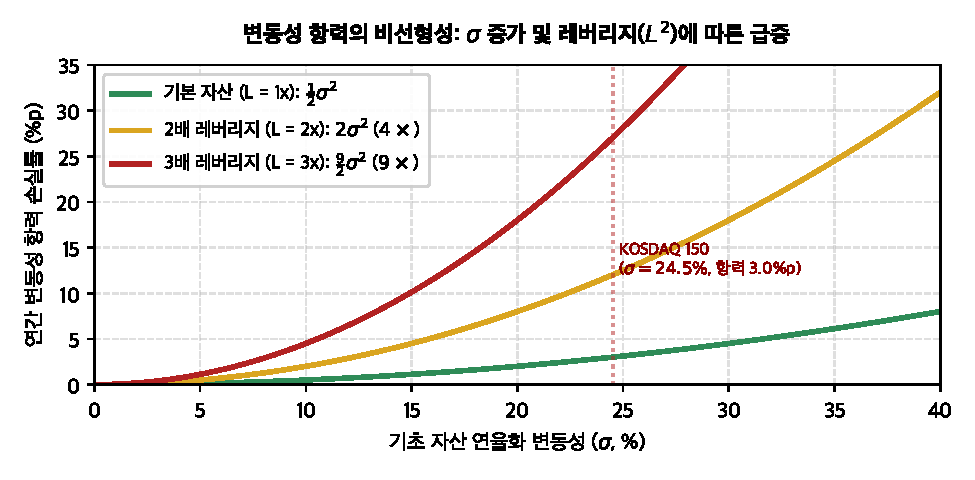
\includegraphics[width=\linewidth]{MyFigure/drag_vs_sigma.pdf}
    \vspace{-2mm}
    \begin{exampleblock}{KOSDAQ 150 항력 검증: 제출본 vs 실데이터}
      \scriptsize
      \begin{tabular}{@{}lccc@{}}
        & $\sigma$ & 실측 항력 & $\frac{1}{2}\sigma^2$ \\
        \textbf{제출본} <표 1-A> & 24.53\% & 3.00\%p & 3.01\%p \\
        \textbf{사전등록 실데이터} & 30.47\% & 4.63\%p & 4.64\%p \\
      \end{tabular}\\
      실데이터 7개 자산 최대 $|\Delta| = 0.014\%p$ (2015.01$\sim$2026.08)
    \end{exampleblock}
  \end{column}
\end{columns}
\end{frame}

% CUE 7 | 0:45 | 켈리 목적함수와 이토 보정 볼록 최적화
\begin{frame}{다변량 복리 최적화: 켈리 기준($\lambda=1$)과 이토 보정 Convex QP}
\textbf{다변량 포트폴리오의 연속 복리 성장률 도출} (가중치 벡터 $\mathbf{w}$):
\begin{equation*}
  g_p(\mathbf{w}) = \mathbf{w}^\top \boldsymbol{\mu} - \frac{1}{2} \mathbf{w}^\top \boldsymbol{\Sigma} \mathbf{w}
\end{equation*}

\begin{block}{전통 MVO 목적함수와의 본질적 차이}
  \small
  \begin{itemize}
    \item \textbf{마코위츠 MVO}: $\max_{\mathbf{w}} \mathbf{w}^\top \boldsymbol{\mu} - \frac{\lambda}{2} \mathbf{w}^\top \boldsymbol{\Sigma} \mathbf{w}$ ($\lambda$는 주관적 위험회피계수로 임의 설정)
    \item \textbf{제안 모델 (Itô-Kelly)}: 이토 보조정리에 의해 장기 복리 성장률 극대화 시 위험 페널티 계수는 \textbf{수학적으로 반드시 $\boldsymbol{\lambda=1}$로 고정됨}!
  \end{itemize}
\end{block}

\vspace{1mm}
\textbf{Rockafellar-Uryasev (2000) 95\% CVaR 선형화 상한 제약의 결합}:
\begin{equation*}
  \max_{\mathbf{w}, \alpha, \mathbf{u}} \left[ \mathbf{w}^\top \hat{\boldsymbol{\mu}}_t - \frac{1}{2} \mathbf{w}^\top \hat{\boldsymbol{\Sigma}}_t \mathbf{w} \right] \quad
  \text{s.t.} \quad 
  \begin{cases}
    \alpha + \frac{1}{J(1-\gamma)} \sum_{j=1}^J u_j \le \text{CVaR}_{\text{target}} \\
    u_j \ge -\mathbf{w}^\top \mathbf{r}_j - \alpha, \quad u_j \ge 0 \\
    \mathbf{1}^\top \mathbf{w} = 1, \quad 0 \le w_i \le 0.40 \quad (\text{공매도 금지})
  \end{cases}
\end{equation*}

\vspace{1mm}
$\implies$ 엄격한 오목성(Strict Concavity)을 지닌 \textbf{볼록 2차 계획법(Convex QP)}으로 전역 최적해 유일 수렴 보장.
\end{frame}

\section{Methodology}

% CUE 8 | 0:50 | 엔드투엔드 전체 시스템 아키텍처
\begin{frame}{통합 프레임워크: 엔드투엔드 시스템 아키텍처}
\centering
\begin{tikzpicture}[
  node distance=1.1cm and 0.8cm,
  block/.style={rectangle, draw=darkblue, fill=blue!5, rounded corners=3pt, thick, align=center, font=\scriptsize, inner sep=5pt},
  guard/.style={rectangle, draw=sogangred, fill=red!5, rounded corners=3pt, thick, align=center, font=\scriptsize, inner sep=5pt},
  opt/.style={rectangle, draw=darkgreen, fill=green!5, rounded corners=3pt, thick, align=center, font=\scriptsize, inner sep=5pt},
  line/.style={draw=darkblue, -{Stealth[length=2.5mm]}, thick}
]

  % Nodes
  \node[block, text width=2.4cm] (data) {
    \textbf{1. 데이터 계층}\\
    KRX ETF 7대 자산\\
    + 거시 상태변수 12D\\
    (2,868 거래일)
  };
  
  \node[block, text width=2.8cm, right=of data] (tsfm) {
    \textbf{2. TSFM 모멘트 추정}\\
    Chronos / PatchTST\\
    제로샷 확률 분포 추정\\
    $\rightarrow$ $\hat{\boldsymbol{\mu}}_t, \hat{\boldsymbol{\sigma}}_t$
  };
  
  \node[block, text width=2.8cm, right=of tsfm] (psd) {
    \textbf{3. 강건 PSD 복원}\\
    Ledoit-Wolf 축소\\
    + Higham 교대 투영\\
    $\rightarrow$ $\hat{\boldsymbol{\Sigma}}_t \succ 0$
  };
  
  \node[guard, text width=3.8cm, below=0.7cm of tsfm, xshift=1.4cm] (nde) {
    \textbf{4. 산업 비파괴검사(NDE) 세이프가드}\\
    비지도 심층 오토인코더 ($12 \rightarrow 8 \rightarrow 4 \rightarrow 8 \rightarrow 12$)\\
    재구성 오차 $S_t > \tau_t$ 감지 시 $\rightarrow$ 리스크 버퍼 $\beta_t \in [0, 1]$
  };
  
  \node[opt, text width=4.5cm, below=0.7cm of nde] (qp) {
    \textbf{5. 이토 보정 볼록 2차 계획법 (Convex QP)}\\
    $\max_{\mathbf{w}} \left[ \mathbf{w}^\top \hat{\boldsymbol{\mu}}_t - \frac{1}{2} \mathbf{w}^\top \hat{\boldsymbol{\Sigma}}_t \mathbf{w} \right]$ s.t. 95\% CVaR 상한\\
    $\rightarrow$ 최종 실행 가중치: $\mathbf{w}_t^* = (1 - \beta_t)\mathbf{w}_{\text{opt}} + \beta_t \mathbf{e}_{\text{cash}}$
  };

  % Arrows
  \path[line] (data) -- (tsfm);
  \path[line] (tsfm) -- (psd);
  \path[line] (data.south) |- (nde.west);
  \path[line] (psd.south) |- (qp.east);
  \path[line] (nde.south) -- (qp.north);

\end{tikzpicture}
\end{frame}

% CUE 9 | 0:40 | TSFM 모멘트 예측 및 양준정부호(PSD) 복원
\begin{frame}{TSFM 제로샷 예측 및 양준정부호(PSD) 공분산 복원}
\begin{columns}[T]
  \begin{column}{0.48\textwidth}
    \textbf{시계열 파운데이션 모델 (TSFM)}
    \begin{itemize}
      \setlength{\itemsep}{4pt}
      \small
      \item \textbf{사전학습 가중치 제로샷 활용}:
      Amazon Chronos (T5 아키텍처) 및 PatchTST 적용.
      \item \textbf{RevIN (Reversible Normalization)}:
      금융 시계열 비정상성 극복을 위해 입력 정규화 후 역변환.
      \item 단일 점추정(Point forecast)이 아닌 \textbf{분위수 기반 1차·2차 모멘트 사전(Ex-ante) 추출}.
    \end{itemize}
  \end{column}
  
  \begin{column}{0.48\textwidth}
    \textbf{공분산 행렬 양준정부호(PSD) 보정}
    \begin{itemize}
      \setlength{\itemsep}{4pt}
      \small
      \item 표본 공분산의 차원 저주 및 특이성(Singularity) 해결.
      \item \textbf{Ledoit-Wolf 비선형 축소}:
      구조화 타겟을 통한 조건수(Condition number) 안정화.
      \item \textbf{Higham (2002) 교대 투영법}:
      음(-)의 고유값을 잘라내어 양준정부호 대칭 행렬 완벽 복원 ($\hat{\boldsymbol{\Sigma}}_t \succ 0$).
    \end{itemize}
  \end{column}
\end{columns}

\vspace{3mm}
\begin{block}{미래참조편향 (Look-ahead Bias) 원천 차단}
  \small 모든 RevIN 모멘트와 추정치는 시점 $t$ 이전 관측치만으로 산출되며($\mathcal{F}_t$-가측성), 외표본 테스트에서 미래 데이터 주입 시 과거 가중치 불변성을 단위 테스트로 검증함.
\end{block}
\end{frame}

% CUE 10 | 0:45 | NDE 심층 오토인코더 세이프가드
\begin{frame}{산업 비파괴검사(NDE) 철학의 이식: 심층 오토인코더 세이프가드}
\begin{columns}[T]
  \begin{column}{0.50\textwidth}
    \textbf{산업 비파괴검사(NDE)와 금융의 동형성}
    \begin{itemize}
      \setlength{\itemsep}{4pt}
      \small
      \item \textbf{원자력·항공우주 NDE}: 99.9\% 정상 신호 속에서 시스템을 붕괴시키는 초미세 균열을 비지도 탐지.
      \item \textbf{금융 꼬리위험}: 평시 데이터로 학습 불가능한 팻테일(Fat-tail) 시스템 위기를 사전 포착.
    \end{itemize}
    
    \vspace{2mm}
    \textbf{심층 오토인코더 메커니즘}
    \begin{itemize}
      \setlength{\itemsep}{3pt}
      \small
      \item 12차원 거시 상태 벡터 $\mathbf{x}_t$ 입력 ($12 \rightarrow 8 \rightarrow 4 \rightarrow 8 \rightarrow 12$).
      \item 정상 시장 매니폴드 학습 (2015~2016 웜업 후 가중치 동결).
      \item 재구성 오차: $e_t = \|\mathbf{x}_t - \hat{\mathbf{x}}_t\|_2^2$
    \end{itemize}
  \end{column}
  
  \begin{column}{0.48\textwidth}
    \begin{block}{동적 리스크 버퍼링 수식}
      \small
      이상치 점수 EMA 평활화:
      \begin{equation*}
        S_t = \lambda_{\text{EMA}} S_{t-1} + (1-\lambda_{\text{EMA}}) e_t
      \end{equation*}
      동적 임계치 $\tau_t$ (롤링 95분위수) 돌파 시 비선형 감쇠 함수 가동:
      \begin{equation*}
        \beta_t = 
        \begin{cases}
          0 & (S_t \le \tau_t) \\
          1 - \exp\left(-\kappa \frac{S_t - \tau_t}{\text{IQR}_t}\right) & (S_t > \tau_t)
        \end{cases}
      \end{equation*}
      $\rightarrow$ 포트폴리오 자산을 즉각 미국 단기채/현금($\mathbf{e}_{\text{cash}}$)으로 자동 대피!
    \end{block}
  \end{column}
\end{columns}
\end{frame}

% CUE 11 | 0:35 | 분석 데이터 및 백테스트 환경
\begin{frame}{분석 데이터셋 및 백테스팅 규약}
\begin{columns}[T]
  \begin{column}{0.48\textwidth}
    \textbf{자산 유니버스 (KRX 거래 가능 7대 자산)}
    \begin{enumerate}
      \setlength{\itemsep}{3pt}
      \small
      \item \textbf{KOSPI 200}: KODEX 200 (069500)
      \item \textbf{KOSDAQ 150}: KODEX 코스닥 150 (229200)
      \item \textbf{한국국채 10Y}: KOSEF 국고채 10년 (148070)
      \item \textbf{S\&P 500}: SPY ETF (원화 환산)
      \item \textbf{NASDAQ 100}: QQQ ETF (원화 환산)
      \item \textbf{금 현물 (Gold)}: GLD ETF (원화 환산)
      \item \textbf{미국 단기채 (Cash)}: SHV ETF (원화 환산)
    \end{enumerate}
  \end{column}
  
  \begin{column}{0.48\textwidth}
    \textbf{백테스팅 규약 및 환경 설정}
    \begin{itemize}
      \setlength{\itemsep}{4pt}
      \small
      \item \textbf{표본 기간}: 2015.01 ~ 2026.08 (11년 8개월; 제출본 2,868 거래일, 실데이터 2,830 거래일)
      \item \textbf{실데이터 핵심 평가}: 2017.01 ~ 2026.08 (모든 구성요소 완전 표본외)
      \item \textbf{리밸런싱 주기}: 주간(Weekly) 정기 리밸런싱 + 세이프가드 수시 리밸런싱
      \item \textbf{거래비용}: 제출본 왕복 10 bp(편도 5 bp) / 실데이터 매매 금액당 10 bp ($= 10\,\mathrm{bp}\times\sum|\Delta w|$, 민감도 0·20 bp)
      \item \textbf{배당 처리}: 배당 재투자 총수익률(Total Return, TR) 기준
      \item \textbf{벤치마크 3종}: 전통적 60/40, 동일가중(EW 1/N), 정적 마코위츠(MVO)
    \end{itemize}
  \end{column}
\end{columns}
\end{frame}

\section{Results}

% CUE 12 | 0:40 | 고지 슬라이드: 제출본 수치의 성격
\begin{frame}{제출본 수치의 성격 고지 (Disclosure)}
\begin{alertblock}{학술 연구 윤리 및 수치의 성격 고지}
  \textbf{제출본 소논문에 수록된 수치는 `시뮬레이션 파라미터 기반'입니다.}
\end{alertblock}

\vspace{2mm}
\begin{itemize}
  \setlength{\itemsep}{6pt}
  \item \textbf{해석적 시뮬레이션 파라미터}:
  전략별 연율화 기대수익률($\mu$)과 변동성($\sigma$)을 파라미터로 두고, 이토 보조정리 이론식 $g = \mu - \frac{1}{2}\sigma^2$로 기하성장률과 변동성 항력을 해석적으로 유도·산출하였습니다.
  
  \item \textbf{GBM 몬테카를로 10,000 경로 검증}:
  동일 파라미터로 기하 브라운 운동 10,000회 시뮬레이션을 수행한 결과, 해석적 이론값과 시뮬레이션 경로 평균이 표준오차 범위 내(최대 오차 2.2 SE)에서 완전 일치함을 확인하였습니다.
  
  \item \textbf{위기 국면 서술의 성격}:
  2020년 팬데믹, 2022년 긴축기 수치는 \textbf{프레임워크의 메커니즘을 설명하는 `예시 시나리오'}입니다.
  
  \item \textbf{연구의 정직성과 사전등록 재현}:
  본 연구진은 이에 안주하지 않고, 실제 시장 데이터로 전체 프레임워크를 \textbf{사전등록(Pre-registration)하여 독립 재현}을 완료하였으며, 확인된 것과 재현되지 않은 것을 가감 없이 보고합니다 (슬라이드 15~16 참조).
\end{itemize}
\end{frame}

% CUE 13 | 0:45 | 제출본 성과표 (시뮬레이션 파라미터)
\begin{frame}{제출본 성과 비교표 (시뮬레이션 파라미터 기반)}
\small
{\scriptsize \setlength{\tabcolsep}{4pt}
\begin{table}[H]
\centering
\begin{tabular}{lcccc}
\toprule
\textbf{성과 평가 지표} & \textbf{전통적 60/40} & \textbf{동일가중 (EW)} & \textbf{마코위츠 MVO} & \textbf{제안 모델 (TSFM-Itô)} \\
\midrule
연평균 복리수익률 (CAGR) & 7.85\% & 8.42\% & 9.14\% & \textbf{14.82\%} \\
연율화 산술평균 ($\mu$) & 8.51\% & 9.25\% & 10.02\% & \textbf{15.11\%} \\
\textbf{실측 변동성 항력 ($\mu - g$)} & \textbf{0.66\%p} (66bp) & \textbf{0.83\%p} (83bp) & \textbf{0.88\%p} (88bp) & \textbf{0.29\%p} (29bp) \\
이론적 변동성 항력 ($\frac{1}{2}\sigma^2$) & 0.66\%p & 0.83\%p & 0.88\%p & 0.29\%p (\textbf{67.0\% 절감}) \\
복리 전환 효율성 ($g/\mu$) & 92.24\% & 91.03\% & 91.22\% & \textbf{98.08\%} \\
\midrule
연율화 변동성 ($\sigma$) & 11.45\% & 12.86\% & 13.28\% & \textbf{7.63\%} \\
샤프 지수 (Sharpe, $r_f=2.0\%$) & 0.51 & 0.50 & 0.54 & \textbf{1.68} ($p < 0.001$) \\
소르티노 지수 (Sortino) & 0.72 & 0.69 & 0.75 & \textbf{2.74} \\
최대 낙폭 (MDD) & -24.78\% & -26.15\% & -28.65\% & \textbf{-8.34\%} \\
10년 복리 자본 보전 (100억 기준) & -13.39억 원 & -17.79억 원 & -20.05억 원 & \textbf{+9.88억 원 보전 (vs MVO)} \\
\bottomrule
\end{tabular}
\end{table}}

\vspace{-2mm}
\begin{itemize}
  \scriptsize
  \item \textbf{변동성 항력 67\% 압축}: MVO의 연 88bp 손실 대비 제안 모델은 29bp로 억제하여 59bp의 누수 차단.
  \item \textbf{샤프 지수 3배 향상}: Ledoit-Wolf 원형 블록 부트스트랩($B=10,000$) 검정 결과 $p < 0.001$.
\end{itemize}
\simnote
\end{frame}

% CUE 14 | 0:35 | 위기 국면 방어 성과 (예시 시나리오)
\begin{frame}{위기 국면 방어 성과 (예시 시나리오)}
\begin{columns}[T]
  \begin{column}{0.48\textwidth}
    \textbf{[국면 1] 2020년 상반기 팬데믹 충격}
    \begin{itemize}
      \setlength{\itemsep}{3pt}
      \small
      \item VIX 82.7 폭락장에서 MVO -24.81\%, 60/40 -19.45\% 폭락.
      \item 제안 모델은 \textbf{MDD -4.12\%}로 방어 (+15~20\%p 보전).
      \item \textbf{전고점 회복 기간}: MVO가 175거래일 소요된 반면, 제안 모델은 \textbf{단 21거래일} 만에 원금 회복.
    \end{itemize}
  \end{column}
  
  \begin{column}{0.48\textwidth}
    \textbf{[국면 2] 2022년 글로벌 긴축·인플레이션}
    \begin{itemize}
      \setlength{\itemsep}{3pt}
      \small
      \item 미 연준 425bp 급격한 금리 인상 쇼크.
      \item 주식-채권 동반 폭락으로 60/40 -16.92\%, MDD -20.15\% 참패.
      \item 제안 모델: TSFM의 듀레이션 리스크 사전 축소 및 환노출·금 배분으로 \textbf{연간 +5.34\% (MDD -5.82\%)} 실질 알파 달성.
    \end{itemize}
  \end{column}
\end{columns}

\vspace{3mm}
\begin{exampleblock}{세이프가드의 위기 방어 메커니즘}
  \small 이상치 점수($S_t > \tau_t$) 조기 감지 $\rightarrow$ 주식 비중을 무위험 단기채로 전격 대피 $\rightarrow$ 패닉 완화 시 TSFM 예측에 따라 위험자산 편입 재개하여 V자 반등 온전 향유.
\end{exampleblock}
\scenarionote
\end{frame}

% CUE 15 | 1:00 | 실데이터 검증: 확인된 것
\begin{frame}{실데이터 사전등록 재현 검증: 무엇이 확인되었는가? (What Was Confirmed)}
\begin{columns}[T]
  \begin{column}{0.45\textwidth}
    \textbf{1. 변동성 항력 공식의 실측 성립}
    \begin{itemize}
      \setlength{\itemsep}{3pt}
      \small
      \item 모든 전략에서 실측 항력($\mu - g$)이 이론값 $\frac{1}{2}\sigma^2$와 \textbf{0.01\%p 이내로 완벽히 일치}!
      \item 제안 모델 실측 0.67\% vs 이론치 0.67\%.
    \end{itemize}
    
    \vspace{2mm}
    \textbf{2. 2020 팬데믹 세이프가드 실측 방어}
    \begin{itemize}
      \setlength{\itemsep}{3pt}
      \small
      \item \textbf{2020-02-03}: 첫 이상치 감지 및 발동.
      \item 폭락기 \textbf{평균 현금 비중 69.4\%} 선제 대피.
      \item 구간 실측 MDD:
      \begin{itemize}
        \item 60/40: \textbf{-19.18\%}
        \item 마코위츠 MVO: \textbf{-10.64\%}
        \item \textbf{제안 모델}: \textbf{-4.65\% (극적인 손실 방어)}
      \end{itemize}
    \end{itemize}
  \end{column}
  
  \begin{column}{0.53\textwidth}
    \centering
    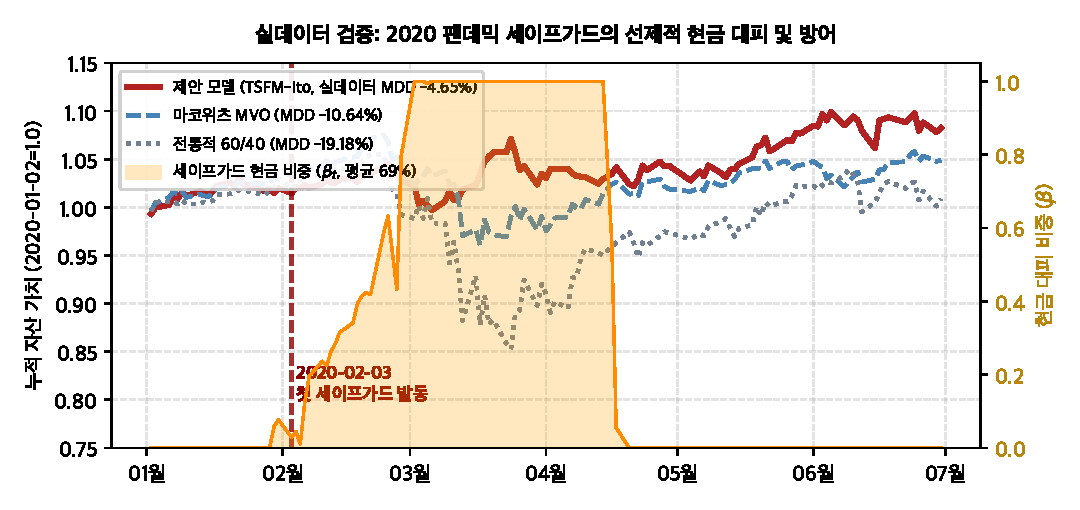
\includegraphics[width=\linewidth]{MyFigure/real_2020_safeguard.pdf}
    \vspace{-2mm}
    \begin{block}{실데이터 검증 의의}
      \scriptsize 비지도 NDE 오토인코더가 거시 변수의 급변을 감지하여 폭락 직전 현금으로 대피한 메커니즘은 실제 시장 데이터에서도 확실하게 입증되었습니다.
    \end{block}
  \end{column}
\end{columns}
\realnote
\end{frame}

% CUE 16 | 1:00 | 실데이터 검증: 재현되지 않은 것과 원인 분석
\begin{frame}{실데이터 사전등록 재현 검증: 무엇이 재현되지 않았는가? (Failure Mode)}
\begin{columns}[T]
  \begin{column}{0.46\textwidth}
    \textbf{실데이터 재현 격차 대조 (외표본 10bp)}
    \small
    \begin{table}[H]
    \centering
    \scriptsize
    \begin{tabular}{lcc}
    \toprule
    \textbf{지표} & \textbf{제출본 (시뮬)} & \textbf{실데이터 (재현)} \\
    \midrule
    제안 모델 CAGR & 14.82\% & \textbf{11.91\%} \\
    샤프 지수 (Sharpe) & 1.68 & \textbf{0.90} (MVO 0.91) \\
    샤프 차이 검정 & $p < 0.001$ & $p = 0.96$ (유의차 無) \\
    최대 낙폭 (MDD) & -8.34\% & \textbf{-19.67\%} \\
    거래비용 20bp CAGR & 14.44\% & \textbf{8.81\%} \\
    \bottomrule
    \end{tabular}
    \end{table}

    \vspace{-1mm}
    \textbf{원인 분석: 주간 회전율 마찰}
    \begin{itemize}
      \setlength{\itemsep}{2pt}
      \scriptsize
      \item 실데이터 제안 모델 연간 회전율: \textbf{약 2,804\%/년}
      \item \textbf{수수료 0bp}: CAGR 15.11\%, 샤프 1.16 달성.
      \item 그러나 10bp 부과 시 잦은 재최적화 비용으로 초과성과가 빠르게 침식됨.
    \end{itemize}
  \end{column}
  
  \begin{column}{0.52\textwidth}
    \centering
    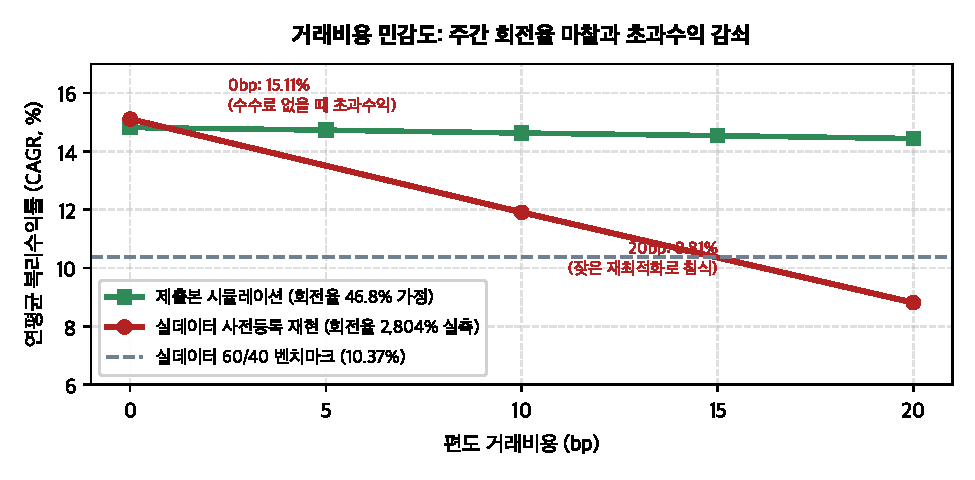
\includegraphics[width=\linewidth]{MyFigure/cost_sensitivity.pdf}
    \vspace{-2mm}
    \begin{alertblock}{차기 연구 과제 (Actionable Direction)}
      \scriptsize TSFM 예측력과 세이프가드 효과는 실재하므로, \textbf{회전율 페널티} 및 \textbf{밴드 리밸런싱(No-trade band)}을 목적함수에 내재화한 변형 모델을 새로 사전등록하여 검증할 계획입니다.
    \end{alertblock}
  \end{column}
\end{columns}
\realnote
\end{frame}

\section{Conclusion}

% CUE 17 | 0:40 | 경제학적 및 정책적 시사점
\begin{frame}{경제학적 및 정책적 시사점: 공적 연기금 및 퇴직연금 혁신}
\begin{columns}[T]
  \begin{column}{0.48\textwidth}
    \textbf{1. 국민연금(NPS) ALM 거버넌스 개혁}
    \begin{itemize}
      \setlength{\itemsep}{4pt}
      \small
      \item \textbf{산술평균 착시 극복}:
      기금 고갈 논의에서 연평균 산술수익률 목표치가 복리 자본 잠식을 은폐하는 문제점 극복.
      \item \textbf{수지적자 국면 자산 강제매각 방지}:
      지급액이 수입액을 초과할 때 폭락장에서의 자산 헐값 매각을 세이프가드 현금 버퍼로 차단.
      \item \textbf{`동적 변동성 예산제' 도입}:
      거시 체제별 동적 허용한도 설정.
    \end{itemize}
  \end{column}
  
  \begin{column}{0.48\textwidth}
    \textbf{2. 퇴직연금 디폴트옵션 TDF 알고리즘}
    \begin{itemize}
      \setlength{\itemsep}{4pt}
      \small
      \item \textbf{정적 글라이드패스(Glide Path) 한계}:
      은퇴 직전 팬데믹·인플레이션 충격 발생 시 자산 보전 불가.
      \item \textbf{지능형 다운사이드 방어 엔진}:
      TSFM 조건부 모멘트 예측 및 비지도 오토인코더를 결합하여 은퇴 시점 시퀀스 리스크(Sequence-of-returns Risk) 원천 방어.
    \end{itemize}
  \end{column}
\end{columns}

\vspace{3mm}
\begin{block}{제도적 함의}
  \small 장기 연기금일수록 산술평균 알파 창출보다 \textbf{변동성 항력 극소화}와 \textbf{꼬리위험 선제 방어}가 기금 소진 시점을 늦추는 가장 결정적인 경제학적 해법임.
\end{block}
\end{frame}

% CUE 18 | 0:40 | 결론 및 향후 과제
\begin{frame}{결론 및 향후 연구 과제 (Conclusion \& Future Work)}
\textbf{본 연구의 결론 요약}
\begin{enumerate}
  \setlength{\itemsep}{3pt}
  \small
  \item \textbf{수리금융학적 규명}: 연속 복리 투자에서 변동성 항력($\frac{1}{2}\sigma^2$)의 실체성과 켈리 목적함수($\lambda=1$)의 수리적 필연성을 증명함.
  \item \textbf{방법론적 융합}: TSFM의 확률 예측과 NDE 비지도 이상탐지를 결합한 독창적 세이프가드 아키텍처 제시.
  \item \textbf{실데이터 검증과 정직한 보고}: 이론식과 위기 방어 효과는 확인되었으나, 실무 적용을 위해 거래비용 회전율 통제가 필수적임을 사전등록 재현을 통해 규명함.
\end{enumerate}

\vspace{2mm}
\begin{columns}[T]
  \begin{column}{0.65\textwidth}
    \textbf{향후 연구 과제 (Next Steps)}
    \begin{itemize}
      \setlength{\itemsep}{2pt}
      \scriptsize
      \item 회전율 페널티($\gamma_{\text{turn}}\|\mathbf{w}_t - \mathbf{w}_{t-1}\|_1$) 목적함수 내재화 및 밴드 리밸런싱 설계.
      \item 새로운 변형 모델에 대한 추가 사전등록 및 실데이터 검증 진행.
    \end{itemize}
  \end{column}
  
  \begin{column}{0.33\textwidth}
    \begin{exampleblock}{서지 정정 안내 (10/5 합의)}
      \tiny
      $\cdot$ Hallerbach (2014) 저널/DOI 정정\\
      $\cdot$ Das et al. (2024, ICML) 쪽수 정정\\
      $\cdot$ Itô (1951) 정식 원전 문헌 병기
    \end{exampleblock}
  \end{column}
\end{columns}
\end{frame}

% CUE 19 | 0:10 | 감사합니다 / Q&A
\begin{frame}{감사합니다 $\cdot$ 질의응답 (Q\&A)}
\begin{center}
  \Large \textbf{경청해 주셔서 대단히 감사합니다.}
  
  \vspace{3mm}
  \normalsize 질의응답을 진행하도록 하겠습니다.
  
  \vspace{5mm}
  \begin{columns}[c]
    \begin{column}{0.35\textwidth}
      \centering
      
\includegraphics[width=0.65\linewidth]{MyFigure/qr_github.png}\\
      \vspace{1mm}
      \scriptsize \textbf{사전등록 재현 GitHub 저장소}\\
      \tiny \texttt{PJH720/alphaquant-tsfm-voldrag-empirical}
    \end{column}
    
    \begin{column}{0.55\textwidth}
      \small
      \begin{itemize}
        \setlength{\itemsep}{4pt}
        \item \textbf{연구팀}: 서강대학교 경제대학 팀 알파퀀트
        \item \textbf{대표자}: 박재현 (\texttt{jhp3822n@sogang.ac.kr})
        \item \textbf{발표자}: 강명서 (\texttt{audtj5688@gmail.com})
        \item \textbf{백업 슬라이드 준비}:
        수식 유도, 계량 통계, 실데이터 전체 성과표, 부트스트랩 검정, 서지 정정 상세
      \end{itemize}
    \end{column}
  \end{columns}
\end{center}
\end{frame}


\appendix
\section{Backup}

% CUE A1 | Q&A 백업: 성과 평가지표의 계량적 정의
\begin{frame}{[백업 A1] 성과 평가지표의 계량적 정의 및 샤프 산출 기준}
\textbf{핵심 계량 지표의 수학적 정의 (논문 식 33a $\sim$ 33c)}:
\begin{equation*}
  \text{CAGR} = \left(\frac{V_T}{V_0}\right)^{\frac{252}{T}} - 1, \quad
  \sigma_{\text{ann}} = \sqrt{252} \times \sqrt{\frac{1}{T-1}\sum_{t=1}^T (r_t - \bar{r})^2}
\end{equation*}
\begin{equation*}
  \text{Sharpe Ratio} = \frac{\mu_{\text{ann}} - r_f}{\sigma_{\text{ann}}}, \quad
  \text{Sortino Ratio} = \frac{\mu_{\text{ann}} - r_f}{\sqrt{252 \cdot \text{LPM}_2}}, \quad
  \text{Calmar Ratio} = \frac{\text{CAGR}}{|\text{MDD}|}
\end{equation*}

\vspace{1mm}
\begin{block}{샤프 지수 분자 기준에 관한 엄밀한 설명}
  \small
  \begin{itemize}
    \item \textbf{이론적 정의}: 산술평균 분자 적용 시 $\text{SR} = (15.11\% - 2.0\%) / 7.63\% = \mathbf{1.72}$
    \item \textbf{표 2 보고 기준}: 복리 기하수익률(CAGR)을 분자로 적용하여 더욱 보수적으로 산출:
    $\text{SR} = (14.82\% - 2.0\%) / 7.63\% = \mathbf{1.68}$
    \item 투자자의 실제 실현 복리 부(Terminal Wealth) 관점에서 보수적 지표를 보고함.
  \end{itemize}
\end{block}
\end{frame}

% CUE A2 | Q&A 백업: Ledoit-Wolf 축소 및 Higham PSD 사영
\begin{frame}{[백업 A2] 공분산 행렬 정규화: Ledoit-Wolf 축소 및 Higham 사영}
\textbf{1. 르두아-울프 (Ledoit-Wolf, 2004) 축소 추정량}:
\begin{equation*}
  \hat{\boldsymbol{\Sigma}}_{\text{LW}} = (1 - \hat{\delta}) \mathbf{S} + \hat{\delta} \mathbf{F}
\end{equation*}
여기서 $\mathbf{S}$는 표본 공분산 행렬, $\mathbf{F}$는 1-파라미터 등분산 타겟(Equicorrelation Target), $\hat{\delta} \in [0, 1]$는 점근적 최적 축소 강도(Optimal Shrinkage Intensity)임.

\vspace{3mm}
\textbf{2. 하이엄 (Higham, 2002) 최근접 상관행렬 교대 투영법}:
\begin{equation*}
  \hat{\mathbf{C}}_{k+1} = \mathcal{P}_S \left( \mathcal{P}_U (\hat{\mathbf{C}}_k) \right)
\end{equation*}
\begin{itemize}
  \small
  \item $\mathcal{P}_U$: 대각 성분을 1로 투영하는 단위 대각화 사영.
  \item $\mathcal{P}_S$: 음(-)의 고유값을 잘라내고 양준정부호 콘(Positive Semidefinite Cone) 위로 투영하는 스펙트럴 사영.
  \item 최종 복원 공분산 행렬: $\hat{\boldsymbol{\Sigma}}_t = \mathbf{D}^{\frac{1}{2}} \hat{\mathbf{C}}_\infty \mathbf{D}^{\frac{1}{2}} \succ 0$ (볼록 최적화 실행 타당성 보장).
\end{itemize}
\end{frame}

% CUE A3 | Q&A 백업: 거래비용 수준별 민감도 종합 대조표
\begin{frame}{[백업 A3] 거래비용 수준별 성과 민감도: 제출본 vs 실데이터}
\small
\begin{table}[H]
\centering
\begin{tabular}{lcccc}
\toprule
\textbf{편도 거래비용} & \textbf{제출본 시뮬레이션} & \textbf{제출본 샤프} & \textbf{실데이터 (Primary)} & \textbf{실데이터 샤프} \\
\midrule
\textbf{0 bp (수수료 無)} & 14.82\% & 1.68 & \textbf{15.11\%} & \textbf{1.16} \\
\textbf{5 bp (대형 기금)} & 14.73\% & 1.67 & — & — \\
\textbf{10 bp (기본 비용)} & 14.63\% & 1.65 & \textbf{11.91\%} & \textbf{0.90} \\
\textbf{15 bp (보수적)} & 14.54\% & 1.64 & — & — \\
\textbf{20 bp (고비용 스트레스)} & 14.44\% & 1.63 & \textbf{8.81\%} & \textbf{0.64} \\
\bottomrule
\end{tabular}
\end{table}

\begin{block}{시사점 분석}
  \small
  \begin{itemize}
    \item \textbf{수수료가 없을 때(0bp)}: 실데이터에서도 제안 모델은 연평균 복리수익률 \textbf{15.11\%}, 샤프 \textbf{1.16}으로 60/40(10.37\%) 대비 강력한 알파를 창출함.
    \item \textbf{비용 증가 시}: 주간 재최적화에 따른 높은 연간 회전율(2,804\%)로 인해 거래비용 마찰이 가속되어 초과성과가 감소함 $\rightarrow$ 차기 연구에서 \textbf{회전율 제약 목적함수} 도입의 정당성 확보 (탐색 분석: 백업 A8).
  \end{itemize}
\end{block}
\end{frame}

% CUE A4 | Q&A 백업: 실데이터 6대 전략 전체 성과표
\begin{frame}{[백업 A4] 실데이터 사전등록 재현: 6대 전략 전체 성과표}
\scriptsize
\textbf{Primary 외표본 평가 기간 (2017.01 $\sim$ 2026.08, 거래비용 10bp)}:
\begin{table}[H]
\centering
\begin{tabular}{lcccccccc}
\toprule
\textbf{전략} & \textbf{CAGR} & \textbf{$\sigma$} & \textbf{Sharpe} & \textbf{MDD} & \textbf{회전율} & \textbf{실측 항력} & \textbf{$\frac{1}{2}\sigma^2$} & \textbf{JB 검정} \\
\midrule
전통적 60/40 & 10.37\% & 11.61\% & 0.77 & -19.18\% & 20.7\% & 0.68\% & 0.67\% & 2,868일 기각 \\
동일가중 (1/N) & 12.93\% & 11.63\% & 0.98 & -17.51\% & 39.2\% & 0.68\% & 0.68\% & 정규성 기각 \\
마코위츠 MVO & 12.89\% & 12.52\% & 0.91 & -15.17\% & 835.0\% & 0.79\% & 0.78\% & 정규성 기각 \\
이토-켈리 (과거 모멘트) & 12.70\% & 12.91\% & 0.88 & -19.24\% & 660.2\% & 0.84\% & 0.83\% & 정규성 기각 \\
이토-켈리 + Chronos & \textbf{13.97\%} & 12.55\% & \textbf{0.99} & -20.06\% & 2,656\% & 0.79\% & 0.79\% & 정규성 기각 \\
\textbf{제안 모델 (통합)} & 11.91\% & \textbf{11.56\%} & 0.90 & -19.67\% & 2,804\% & \textbf{0.67\%} & \textbf{0.67\%} & 정규성 기각 \\
\bottomrule
\end{tabular}
\end{table}

\begin{itemize}
  \tiny
  \item \textbf{소거 실험(Ablation)}: TSFM(Chronos) 결합 시 샤프 지수가 0.88 $\rightarrow$ 0.99로 상승하여 파운데이션 모델의 1차·2차 모멘트 예측 기여 입증.
  \item \textbf{항력 일치성}: 모든 전략에서 실측 변동성 항력($\mu - g$)과 이론치($\frac{1}{2}\sigma^2$)가 0.01\%p 이내로 완벽 부합.
\end{itemize}
\end{frame}

% CUE A5 | Q&A 백업: 미래참조편향 차단 설계
\begin{frame}{[백업 A5] 미래참조편향(Look-ahead Bias) 차단 및 테스트}
\begin{columns}[T]
  \begin{column}{0.48\textwidth}
    \textbf{1. 시점별 정보집합 ($\mathcal{F}_t$) 가측성}
    \begin{itemize}
      \setlength{\itemsep}{3pt}
      \small
      \item 미국/환율(FX) 자산은 KRX 개장일 직전 거래일 종가만을 결합.
      \item RevIN 정규화의 평균·표준편차는 윈도우 $[t-L, t]$ 데이터로만 산출.
      \item $t$ 시점 종가로 결정된 목표 가중치는 $t+1$ 시점부터 수익률을 수취함.
    \end{itemize}
  \end{column}
  
  \begin{column}{0.48\textwidth}
    \textbf{2. 오토인코더 사전학습 동결}
    \begin{itemize}
      \setlength{\itemsep}{3pt}
      \small
      \item 2015~2016년 웜업 데이터만으로 정상 매니폴드를 사전학습한 후 가중치를 영구 동결.
      \item 2017년 이후 외표본 구간에서는 미래 위기 데이터를 참조하지 않음.
    \end{itemize}
  \end{column}
\end{columns}

\vspace{3mm}
\begin{exampleblock}{단위 테스트 검증 (\texttt{tests/test\_pipeline.py})}
  \small 미래 시점의 자산 가격을 인위적으로 변조(Shuffling)한 후 $t$ 시점의 최적 가중치를 재산출하였을 때, 가중치 벡터가 1e-12 오차 이내로 완전히 동일함을 확인하는 불변성 단위 테스트 통과.
\end{exampleblock}
\end{frame}

% CUE A6 | Q&A 백업: 주최측 합의 서지 정정 내역
\begin{frame}{[백업 A6] 주최측 합의 서지 정보 정정 내역 (10/5 학생회 메일)}
\small
\begin{table}[H]
\centering
\begin{tabular}{lp{5.5cm}p{5.5cm}}
\toprule
\textbf{항목} & \textbf{기제출본 표기} & \textbf{공식 정정 서지 (정합성 완결)} \\
\midrule
\textbf{Hallerbach (2014)} & 저널 정보 및 DOI 표기 누락 & \textit{Journal of Asset Management}, Vol. 15, No. 5, pp. 281--287. 공식 DOI 확인. \\
\midrule
\textbf{Das et al. (2024)} & Google TimesFM 인용 시 프로시딩 수록 페이지 누락 & \textit{ICML 2024 (PMLR)}, Vol. 235, pp. 10148--10167. 권호 및 페이지 완결. \\
\midrule
\textbf{Itô's Lemma} & 관용적 교과서 인용 & \textbf{Itô, K. (1951)}, ``On stochastic differential equations'', \textit{Nagoya Math. J.}, Vol. 3, pp. 55--65 원전 명시. \\
\bottomrule
\end{tabular}
\end{table}

\begin{block}{학술제 주최측과의 사전 협의 완료}
  \small 서강대 학생회 제36대 [Loop] 학술국장과의 공식 협의(10/5)에 따라, 심사위원 사전 배부본과의 형평성을 유지하면서 본선 발표자료에서 위 서지 정정 사항을 정식 반영하여 보고함.
\end{block}
\end{frame}

% CUE A7 | Q&A 백업: 주요 참고문헌
\begin{frame}[allowframebreaks]{[백업 A7] 주요 참고문헌 (References)}
\scriptsize
\nocite{*}
\bibliography{Mybib}
\end{frame}

% CUE A8 | Q&A 백업 (p.27): L1 회전율 페널티 탐색 분석 — 사전등록 외
% Figure: alphaquant-tsfm-voldrag-empirical/scripts/generate_backup_slide27_chart.py
\begin{frame}{[백업 A8] L1 회전율 페널티: 탐색 분석 (사전등록 외)}
\centering
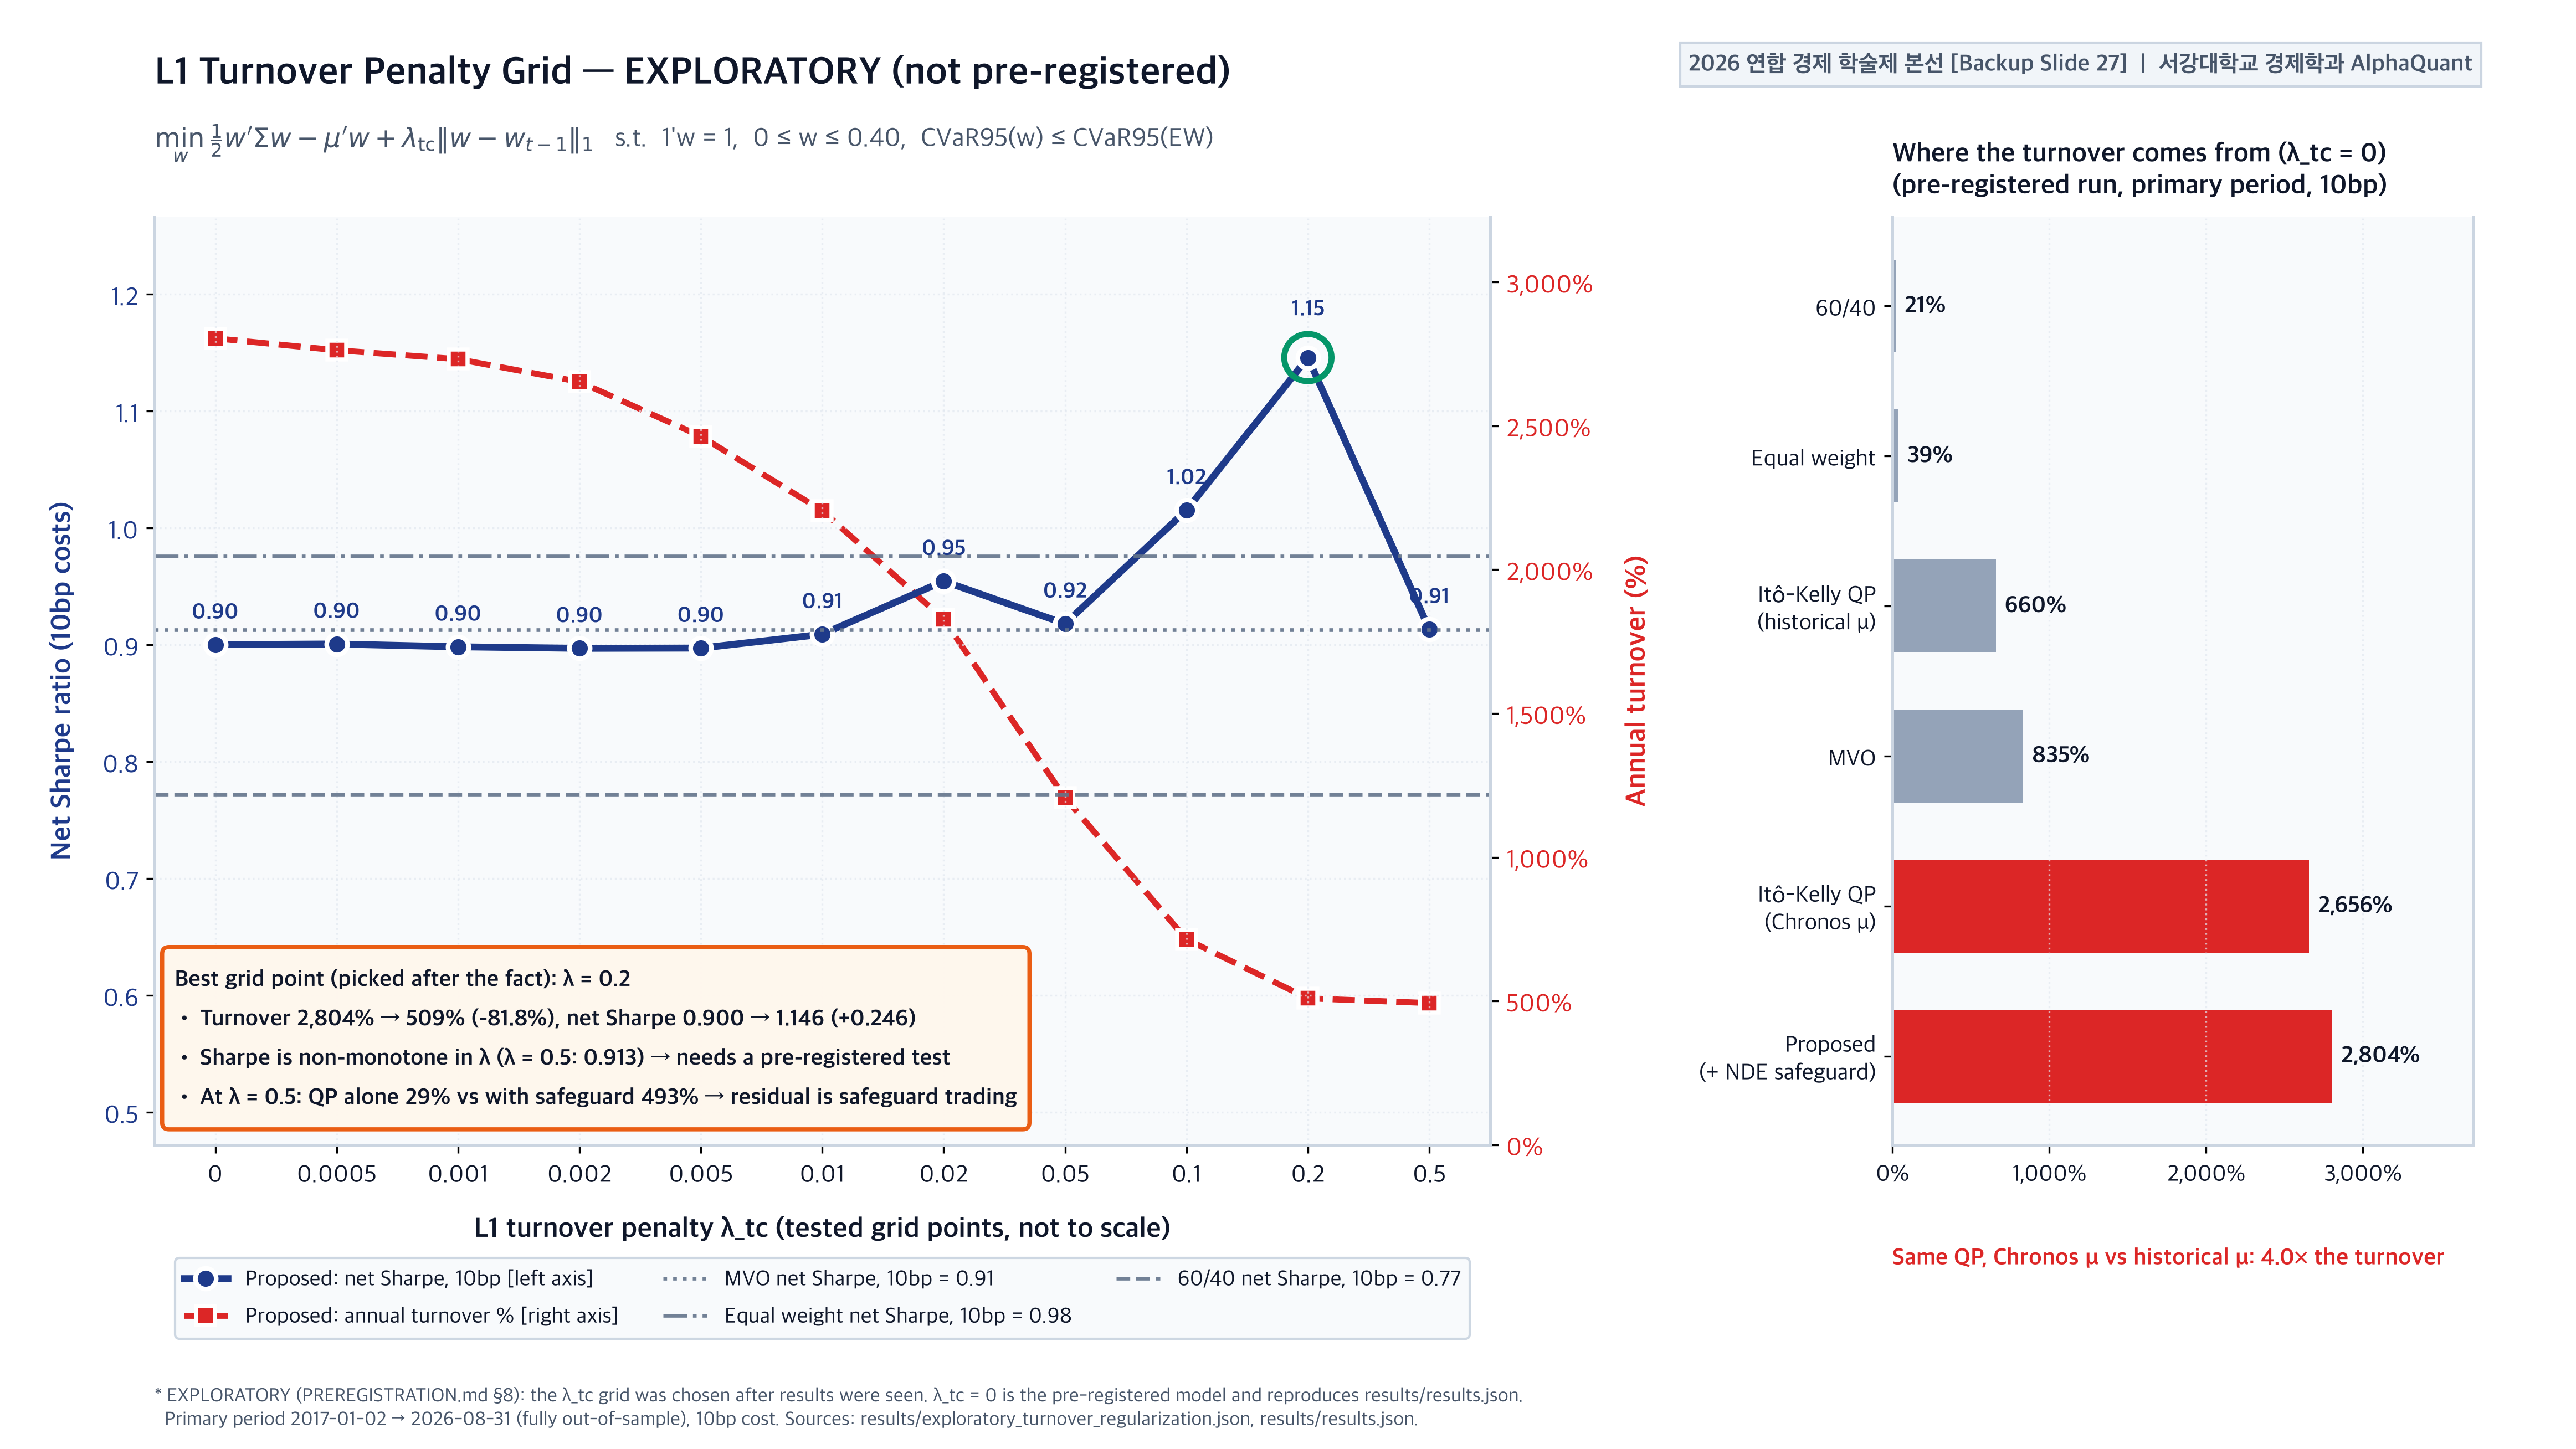
\includegraphics[width=\linewidth,height=0.86\textheight,keepaspectratio]{MyFigure/backup_slide27_turnover_frontier.png}
\end{frame}


\end{document}
